\question{
  \item Suponha que um determinado protocolo da camada da ligação de dados usa um código
  cíclico de verificação, CRC, gerado pelo polinómio gerador $G(x) = x^4 + x^3 + 1$.
}

\begin{enumerate}[leftmargin=\labelsep]
  \subquestion{
  \item Determine os bits de CRC do bloco de dados $00111011001$.
        }

        Com um polinómio gerador do tipo $x^4 + x^3 + 1$, sabemos que o divisor pretendido
        será, em binário, $11001$. O dividendo, $00111011001$, vê concatenados quatro zeros
        à direita (são sempre concatenados $N - 1$ zeros, onde $N$ é o número de bits do
        divisor). A divisão será feita por subtrações sucessivas, e o resultado será o resto
        da divisão. A divisão é feita da seguinte forma:

        \begin{figure}[H]
          \centering
          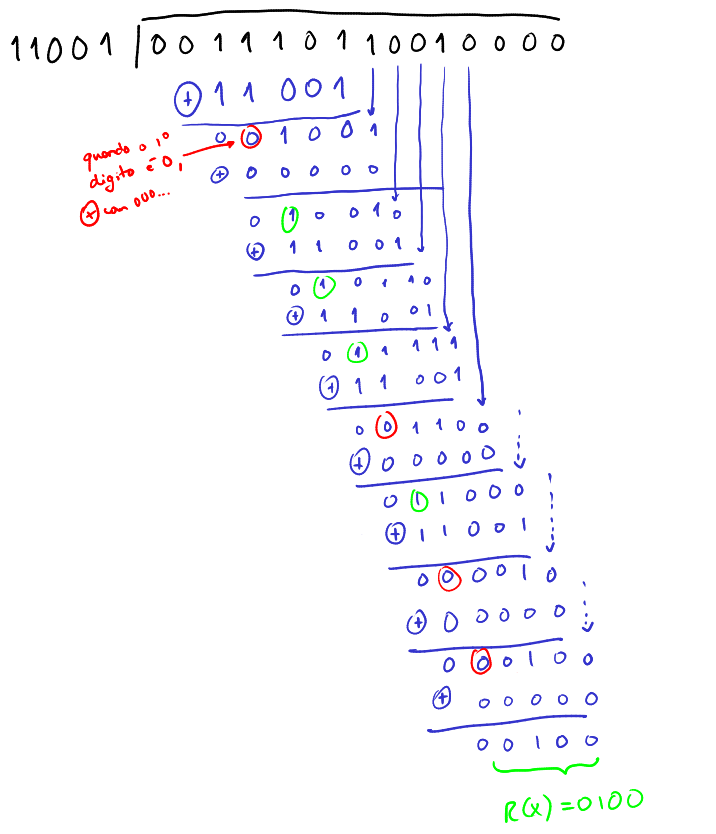
\includegraphics[width=0.4\textwidth]{assets/014a.png}
        \end{figure}

        \subquestion{
  \item Suponha que o emissor forma uma trama com o bloco de dados e os bits de CRC
        da alínea anterior. A trama é enviada do emissor para o recetor, é corrompida no
        canal que os une, e é recebida pelo recetor na forma $001110110000110$. Os erros
        são detetados no recetor?
        }

        Um erro será detetado na mensagem caso o que seja recebido não for divisível pelo
        polinómio gerador.

        \begin{figure}[H]
          \centering
          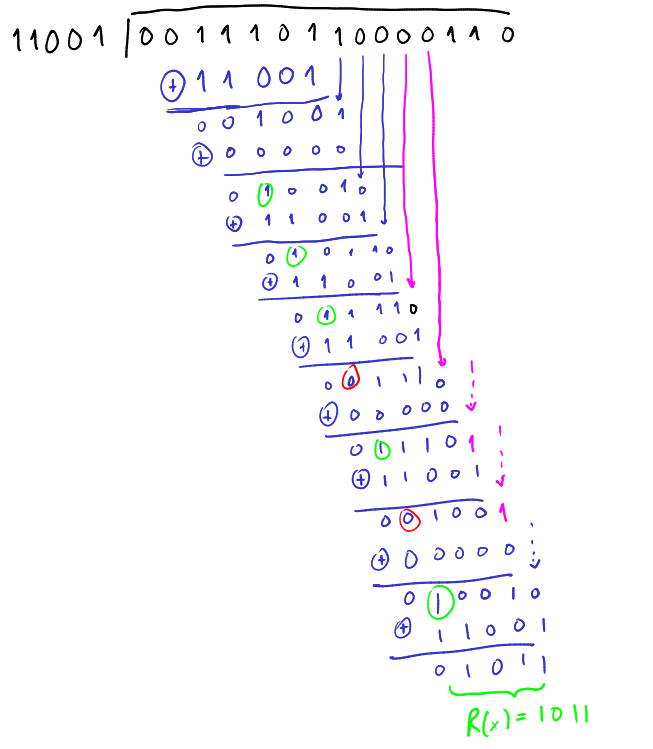
\includegraphics[width=0.4\textwidth]{assets/014b.png}
        \end{figure}

        Podemos, assim, concluir que o erro é detetado, já que $R(x) \neq 0$.
\end{enumerate}